\section{System Overview}
\label{sec:systemOverview}



The objective of the system is to detect and segment roads found in aerial color images by supervised learning. A supervised learning algorithm that works well for images is a \ac{CNN}, and has therefore been chosen for this task. \ac{CNN}s have been applied to many computer vision tasks lately, with results outperforming other approaches \citep{Krizhevsky_imagenet}. As discussed in Section \ref{sec:background_theory}, these networks reduce the need for feature engineering by having the network learn suitable feature detectors, which is crucial \todo{crucial to strong of a word?} for tasks involving images. Additionally, an important part of creating a competent road detection system from supervised learning, is by having a large dataset containing aerial images and label images showing exactly which pixels represent roads.\\

\begin{figure}[t]
\begin{center}
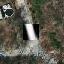
\includegraphics[width=0.15\columnwidth]{figs/labeloverlay.png}
\caption[Patches]{output prediction patch superimposed on input aerial image patch}
\label{fig:system_data_patch}
\end{center}
\end{figure}

The system shares many similarities to the patch-based deep neural network presented by \cite{Mnih_aerial_images_noisy}. The system produces a patch of predictions given a patch of pixel values, where each value indicate the probability of the input pixel depicting a road. Given a $64 \times 64$ aerial image patch the system compute a $16 \times 16$ patch of probabilities. The probabilities indicate the presence of road for the pixels found in the center of the aerial image patch. An example of input image patch and the output prediction patch can be seen in Figure \ref{fig:system_data_patch}.  \\

\begin{figure}[t]
\begin{center}
\includegraphics[width=1\columnwidth]{figs/system_overview.png}
\caption[Components of the system]{Components of the system}
\label{fig:system_components}
\end{center}
\end{figure}

The actual implementation consists of two primary components, and an optional storage and graphical user interface web server component. The components and how they related, can be seen in Figure \ref{fig:system_components}. The storage and user interface component is not integral to the task of road detection, but has been a helpful aid when conducting experiments. Additionally, the patch dataset creator component is interchangeable, and can easily accommodate other varieties of segmentation datasets. In relation to the research questions the patch dataset creator component is altered when investigating curriculum learning, and the loss function of the \ac{CNN} component is replaced when bootstrapping loss is applied. \\


